\documentclass[a4j]{celb-report}
%%%
%%% 計算機工学実験Bレポートテンプレート
%%%  このテンプレートを使う場合,celb-report.clsとjlisting.styが必要です.
%%%  このファイルと同じディレクトリに置いておいてください.
%%%

%%%
%%% まずはここで各種設定
%%%
\usepackage{comment}
\period{2} % ← 何回目のレポートか(1~3)
\stunum{S153012} % ← 学生番号
\author{伊藤 太清} % ← 学生氏名
\date{\today} % ← レポート提出日

\begin{document}

\maketitle

%%%%%%%%%%%%%%%%%%%%%%%%%%%%%%%%%%%%%%%%%%%%%%%%%%%%%%%%%%%%%%%%%%%%%
% レポート作成の手引:
%   レポート提出時は、ここから「レポート作成の手引ここまで」までの行をすべて削除すること!
%%%%%%%%%%%%%%%%%%%%%%%%%%%%%%%%%%%%%%%%%%%%%%%%%%%%%%%%%%%%%%%%%%%%%
\begin{comment}
\setcounter{section}{-1}
\section{レポート作成の手引}

各レポート,対応する回ごとに章(\verb|\section|)に分け,テキストの報告内容にて指示されている課題ごとに節(\verb|\subsection|)を用意して記載する.次章にて第1回分の例を記載しているので,適宜参考にすること.

% ----------------------------------------------------
\subsection{プログラムのソースコード,実行結果等を掲載する場合}

プログラムのソースコードや実行結果等を貼り付ける場合は,\verb|\lstlisting|環境を用いると良い.使い方は,このファイルの\texttt{tex}ソースを参考にすること.基本的には,ソースに記載の内容をコピーし,実行結果を書き換えると良い.
%
% --- 実行結果ここから
\begin{lstlisting}[basicstyle=\ttfamily\footnotesize, frame=single]

※※ ここに実行結果を貼り付ける. ※※
 
\end{lstlisting}
% --- 実行結果ここまで
%

% ----------------------------------------------------
\subsection{課題}

各回で用意されている考察・調査課題については,\verb|\kadai|を用いて,課題文と回答を記載する.第1回分の例を参考にすること.

% ----------------------------------------------------
\subsection{図の貼り付け}

図を貼り付ける場合は,\verb|\figure|環境を用いる.基本的には,このファイルの\texttt{tex}ソース内にある記述をそのまま用いれば良い.\verb|\includegraphcs|で画像ファイルを指定し,\verb|\caption|で図にキャプションを付ける.\verb|\label|は,本文中で図番号を参照するために付けておくラベルである(詳しくは後述).
%
\begin{figure}[htb]
 \centering 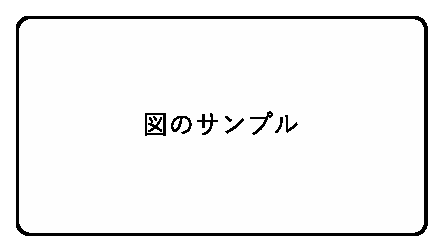
\includegraphics[scale=0.8]{sample-figure.eps}
 \caption{図のサンプル} \label{fig:sample}
\end{figure}
%

本文中で図を引用する場合は,図中で指定した\verb|label|を\verb|\ref|を用いて参照する.例えば上図で\verb|\label{fig:sample}|としている状態で本文中に``図\verb|\ref{fig:sample}|''と記述すると,texコンパイル後のファイルでは当該箇所が``図\ref{fig:sample}''に変換される.``図??''となる場合は,もう1度texコンパイルしてみて,それでも参照がされない場合は,ラベルが一致しているかどうか確認する.

% ----------------------------------------------------
\subsection{(第3レポートのみ)グループ内の役割分担}

第3レポートの対象となる回では,複数人のグループで作業を行うため,各回で誰が何を担当したのかも節(\verb|\subsection|)を用いて記載する.以下は記載例である.\texttt{tex}ソースに記載の通り,\verb|\description|環境を用いると良い.
%
\begin{description}
 \item[s123456 学生 なまえ] ネットワークの配線,環境の構築
 \item[s135791 相方 ひとりめ] プログラムのコーディング,デバッグ
 \item[s246802 相方 ふたりめ] コーディングのサポート
 \item[s369258 相方 さんにんめ] 3人の応援
\end{description}

% ----------------------------------------------------
\subsection{参考文献等}

書籍,インターネット上の情報などを参考にした場合,対象となるすべての回のものをまとめて,\verb|\thebibliography|環境を用いて出展を明記する.書き方は本ファイルの\texttt{tex}ソースを参考にする.
%
%%%%%%%%%%%%%%%%%%%%%%%%%%%%%%%%%%%%%%%%%%%%%%%%%%%%%%%%%%%%%%%%%%%%%
% レポート作成の手引ここまで
%%%%%%%%%%%%%%%%%%%%%%%%%%%%%%%%%%%%%%%%%%%%%%%%%%%%%%%%%%%%%%%%%%%%%


%%%%%%%%%%%%%%%%%%%%%%%%%%%%%%%%%%%%%%%%%%%%%%%%%%%%%%%%%%%%%%%%%%%%%
% 第1回分(第1レポート内)サンプル
%   第1レポートでは,第1回~第4回分それぞれを 章 (\section) として1つのレポートにまとめること
%%%%%%%%%%%%%%%%%%%%%%%%%%%%%%%%%%%%%%%%%%%%%%%%%%%%%%%%%%%%%%%%%%%%%
%%% ------------------------------------------------------------------
\newpage % ← 改ページ
\section{第1回 誤り制御符号(1):パリティ符号}

% ----------------------------------------------------
\subsection{実行結果}

%
% --- 実行結果ここから
\begin{lstlisting}[basicstyle=\ttfamily\footnotesize, frame=single]
$ ./parity



...


 
\end{lstlisting}
% --- 実行結果ここまで
%

\subsection{実行結果に対する考察}
前節の実行結果より,~であることがわかる.また,~であるものと考えられる.


% ----------------------------------------------------
\subsection{課題}

\kadai{今回の実験で作成したパリティ符号は,偶数パリティと奇数パリティのいずれであるかを答えよ.}

~~~であるため,◯数パリティである.

\kadai{1ビット水平パリティ符号について調査せよ.}

1ビット水平パリティ符号とは,~~ものである.~~.

\kadai{1ビット水平パリティ符号と1ビット垂直パリティ符号を組み合わせることにより,1ビットの誤りを訂正できることを示せ.}

~~.

以上より,1ビット水平パリティ符号と~~~,~~~できる.
\end{comment}
%
%%%%%%%%%%%%%%%%%%%%%%%%%%%%%%%%%%%%%%%%%%%%%%%%%%%%%%%%%%%%%%%%%%%%%
% 第1回分サンプルここまで
%%%%%%%%%%%%%%%%%%%%%%%%%%%%%%%%%%%%%%%%%%%%%%%%%%%%%%%%%%%%%%%%%%%%%

%%% ------------------------------------------------------------------
\newpage
\section{第5回 TPCソケットの基礎}
\subsection{プログラムの実行結果}
\subsection{プログラムの改造}

....

%%% ------------------------------------------------------------------
\newpage
\section{第x回 実験タイトル}

....

%%% ------------------------------------------------------------------
% --- 参考文献リストここから
\newpage
\begin{thebibliography}{9}
\begin{comment}
\bibitem{book-sample} 神崎映光,西川津ビビッド,出雲島猫,「書籍の参照はこんな感じ」,島大出版,1979年.
\bibitem{url-sample} 島根大学 総合理工学部 数理・情報システム学科(情報系),http://www.cis.shimane-u.ac.jp/.
\end{comment}
\end{thebibliography}
% --- 参考文献リストここまで
%

\end{document}
